\section{Clustering}\label{bg:clustering}\note{Should maybe be moved to description of collaborative filtering}
Clustering is a widely used method when working with a large amount of data. In short it is about grouping similar data in ``clusters''. In the domain of recommending clustering is commonly used together with the recommendation method called collaborative filtering, where the data is clustered into users with similar ratings for given items. The user data in these clusters are then used to make individual recommendations to the users.

One of the most efficient collaborative filtering methods which uses clustering is matrix factorization, described in \sectionref{bg:matrixfactorization}. 

Looking at the dataset we get when we have to make group recommendations, it is rather small compared to what is used in normal group recommenders.

Although using clustering in general give some good results, clustering when recommending to groups is not the most suitable solution, unless the group members are compared to a large database of users, where clustering becomes a decent if not great method to improve the execution time of the comparison.

When using clustering for recommendation systems typically they are used in collaborative filtering to find users with similar interests and predict new items based on users in the same clusters. However we initially thought of using clustering in another way. Starting with the individual members, as seen on Figure \ref{fig:bg:clustering_1}, we wanted to group them together in small groups and treat them as if they were one user, as seen on Figure \ref{fig:bg:clustering_2}. This way the aggregations can be performed on smaller groups with the intend to make the aggregation faster. The grouping does not need to stop after just one iteration but can be continued, as seen on Figure \ref{fig:bg:clustering_3}. However the size of the groups intended to benefit from the recommender is not large enough to get a significant impact from using this method. \todo{Make the figures smaller}

\begin{figure}[H]
	\centering
	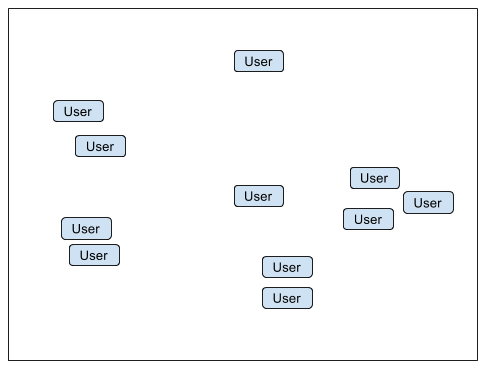
\includegraphics[scale=0.6]{graphics/Clustering_1.png}
	\caption{Initial members of the group in a graphical representation of how similar they are to each other.}
	\label{fig:bg:clustering_1}
\end{figure}

\begin{figure}[H]
	\centering
	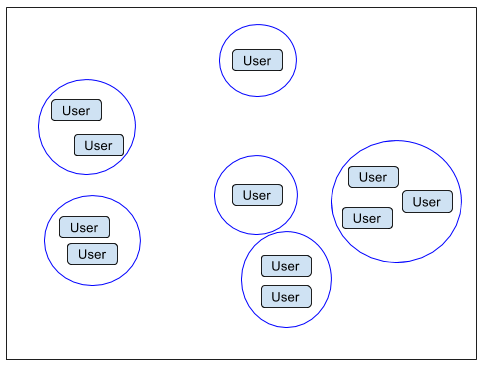
\includegraphics[scale=0.6]{graphics/Clustering_2.png}
	\caption{The members have been grouped together with those they resemble most, indicated by the blue rings.}
	\label{fig:bg:clustering_2}
\end{figure}

\begin{figure}[H]
	\centering
	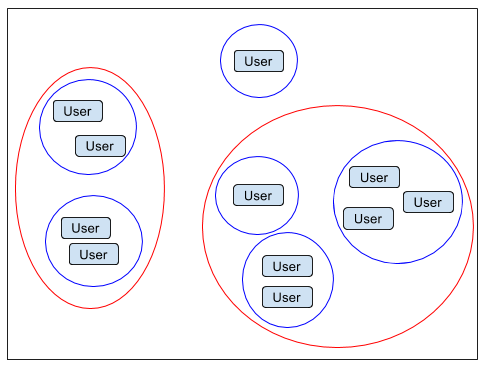
\includegraphics[scale=0.6]{graphics/Clustering_3.png}
	\caption{Groupings of members are grouped together in larger groupings, indicated by the red rings.}
	\label{fig:bg:clustering_3}
\end{figure}